\iffalse
\title{CE-2011-1-13}
\author{EE24BTECH11036 - Krishna Patil}
\section{ce}
\chapter{2011}
\fi
\item Let \cbrak{A}  be a square matrix which is neither symmetric nor skew-symmetric, and  ${\cbrak{A}}^{T}$ is its transpose . The sum and difference of these matrices are defined as $\cbrak{S} = \cbrak{A} + {\cbrak{A}}^{T}$  and  $\cbrak{D} = \cbrak{A} - {\cbrak{A}}^{T}$, respectively. Which of the following statements is TRUE?
\begin{enumerate}
\item Both $\cbrak{S}$ and $\cbrak{D}$ are symmetric 
\item Both $\cbrak{S}$ and $\cbrak{D}$ are skew-symmetric
\item $\cbrak{S}$ is skew-symmetric and $\cbrak{D}$ is symmetric
\item $\cbrak{S}$ is symmetric and $\cbrak{D}$ is skew-symmetric
\end{enumerate}
\item The square root of a number $N$ is to be obtained by applying the Newton Raphson iterations to the equation $x^2 - N = 0$. If $i$ denotes the iteration index, the correct iterative scheme will be
\begin{enumerate}
    \item $x_{i+1} = \frac{1}{2} \brak{x_i + \frac{N}{x_i}}$
\item $x_{i+1} = \frac{1}{2} \brak{x_i^2 + \frac{N}{x_i}}$
\item $x_{i+1} = \frac{1}{2} \brak{x_i + \frac{N^2}{x_i}}$
\item $x_{i+1} = \frac{1}{2} \brak{x_i - \frac{N}{x_i}}$
\end{enumerate}
\item There are two containers, with one containing 4 Red and 3 Green balls and the other containing 3 Blue and 4 Green balls. One ball is drawn at random from each container. The probability that one of the balls is Red and the other is Blue will be
\begin{enumerate}
\begin{multicols}{2}
\item $\frac{1}{7}$
\item $\frac{9}{49}$
\item $\frac{12}{49}$
\item $\frac{3}{7}$
\end{multicols}
\end{enumerate}
\item For the fillet weld of size $s$ shown in the adjoining figure, the effective throat thickness is \\
\begin{tikzpicture}
\fill[gray!20] (-1,0) rectangle (6,-0.3);
\begin{scope}[rotate=9, shift={(2.5,-0.5)}]
\fill[gray!40] (0,0) rectangle (0.3,3.5);
\end{scope}
\fill[pattern=north east lines] (3.2,-0.2) arc[start angle=0, end angle=99, radius=0.7];
\draw[thick,->] (2.7,0) ++(0.6,0) arc[start angle=0, end angle=99, radius=0.6];
\node at (3.6,0.8) {$99^\circ$};
\node at (2.9,-0.25) {$s$};
\node at (2.25,0.25) {$s$};
\node[below right] at (3.3,0.2) {Fillet weld};
\end{tikzpicture}
\begin{enumerate}
\begin{multicols}{2}
\item $0.61s$ 
\item $0.65s$
\item $0.70s$
\item $0.75s$
\end{multicols}
\end{enumerate}
\item A $16$ mm thick plate measuring $650 \text{mm} \times 420 \text{mm} $ is used as a base plate for an ISHB $300$ column subjected to a factored axial compressive load of $2000  \text{kN}$. As per IS $456-2000$, the minimum grade of concrete that should be used below the base plate for safely carrying the load is
\begin{enumerate}
\begin{multicols}{2}
\item $ M15 $
\item $ M20 $
\item $ M30 $
\item $ M40 $
\end{multicols}
\end{enumerate}
\item Consider a reinforcing bar embedded in concrete. In a marine environment this bar undergoes uniform corrosion, which leads to the deposition of corrosion products on its surface and an increase in the apparent volume of the bar. This subjects the surrounding concrete to expansive pressure. As a result, corrosion induced cracks appear at the surface of concrete. Which of the following statements is TRUE?
\begin{enumerate}

\item Corrosion causes circumferential tensile stresses in concrete and the cracks will be parallel to the corroded reinforcing bar.
\item Corrosion causes radial tensile stresses in concrete and the cracks will be parallel to the corroded reinforcing bar.
\item Corrosion causes circumferential tensile stresses in concrete and the cracks will be perpendicular to the direction of the corroded reinforcing bar.
\item Corrosion causes radial tensile stresses in concrete and the cracks will be perpendicular to the direction of the corroded reinforcing bar.
\end{enumerate}
\item The results for sieve analysis carried out for three types of sand, \brak{ P }, \brak{ Q } and \brak{ R }, are given in the adjoining figure. If the fineness modulus values of the three sands are given as \brak{ \text{FM}_P }, \brak{ \text{FM}_Q } and \brak{ \text{FM}_R }, it can be stated that
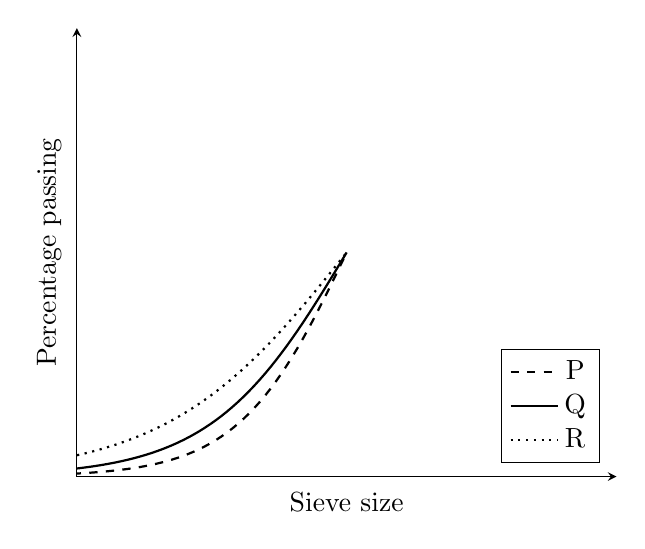
\begin{tikzpicture}
\begin{axis}[
    xlabel={Sieve size},
    ylabel={Percentage passing},
    axis lines=left,
    ymin=0, ymax=100,
    xmin=0, xmax=10,
    legend pos=south east,
    samples=100,
    xtick=\empty,
    ytick=\empty
   ]
\addplot[thick, dashed] {100/(1 + exp(-1*(x-5)))}; \addlegendentry{P}
\addplot[thick] {100/(1 + exp(-0.8*(x-5)))}; \addlegendentry{Q}
\addplot[thick, dotted] {100/(1 + exp(-0.6*(x-5)))}; \addlegendentry{R}
\end{axis}
\end{tikzpicture}
\begin{enumerate}
\begin{multicols}{2}
\item $ \text{FM}_Q = \sqrt{\text{FM}_P \times \text{FM}_R} $
\item $ \text{FM}_Q = 0.5 \, (\text{FM}_P + \text{FM}_R) $
\item $ \text{FM}_P > \text{FM}_Q > \text{FM}_R $
\item $ \text{FM}_P < \text{FM}_Q < \text{FM}_R $
\end{multicols}
\end{enumerate}
\newpage
\item The cross-section of a thermo-mechanically treated (TMT) reinforcing bar ha
\begin{enumerate}
\item soft ferrite-pearite throughout .
\item hard martensite throughout.
\item a soft ferrite-pearite core with a hard martensitic rim.
\item a hard martensite core with a soft pearite-bainitic rim.
\end{enumerate}
\item Consider a simply supported beam with a uniformly distributed load having a neutral axis \brak{NA} as shown. For points $ P $  (on the neutral axis) and $ Q $ (at the bottom of the beam) the state of stress is best represented by which of the following pairs?
\begin{figure}[!ht]
\centering
\resizebox{1\textwidth}{!}{%
\begin{circuitikz}
\tikzstyle{every node}=[font=\normalsize]
\draw  (5.5,15.75) rectangle (13.5,13.75);
\draw [dashed] (4.5,14.75) -- (14.75,14.75);
\node [font=\normalsize] at (15.25,14.75) {NA};
\draw [line width=0.5pt, short] (5.5,16.5) -- (13.5,16.5);
\draw [line width=0.5pt, ->, >=Stealth] (5.5,16.5) -- (5.5,15.75);
\draw [line width=0.5pt, ->, >=Stealth] (5.75,16.5) -- (5.75,15.75);
\draw [line width=0.5pt, ->, >=Stealth] (6,16.5) -- (6,15.75);
\draw [line width=0.5pt, ->, >=Stealth] (6.25,16.5) -- (6.25,15.75);
\draw [line width=0.5pt, ->, >=Stealth] (6.5,16.5) -- (6.5,15.75);
\draw [line width=0.5pt, ->, >=Stealth] (6.75,16.5) -- (6.75,15.75);
\draw [line width=0.5pt, ->, >=Stealth] (7,16.5) -- (7,15.75);
\draw [line width=0.5pt, ->, >=Stealth] (7.5,16.5) -- (7.5,15.75);
\draw [line width=0.5pt, ->, >=Stealth] (7.25,16.5) -- (7.25,15.75);
\draw [line width=0.5pt, ->, >=Stealth] (7.75,16.5) -- (7.75,15.75);
\draw [line width=0.5pt, ->, >=Stealth] (8,16.5) -- (8,15.75);
\draw [line width=0.5pt, ->, >=Stealth] (8.25,16.5) -- (8.25,15.75);
\draw [line width=0.5pt, ->, >=Stealth] (8.5,16.5) -- (8.5,15.75);
\draw [line width=0.5pt, ->, >=Stealth] (8.75,16.5) -- (8.75,15.75);
\draw [line width=0.5pt, ->, >=Stealth] (9,16.5) -- (9,15.75);
\draw [line width=0.5pt, ->, >=Stealth] (9.25,16.5) -- (9.25,15.75);
\draw [line width=0.5pt, ->, >=Stealth] (9.5,16.5) -- (9.5,15.75);
\draw [line width=0.5pt, ->, >=Stealth] (9.75,16.5) -- (9.75,15.75);
\draw [line width=0.5pt, ->, >=Stealth] (10,16.5) -- (10,15.75);
\draw [line width=0.5pt, ->, >=Stealth] (10.25,16.5) -- (10.25,15.75);
\draw [line width=0.5pt, ->, >=Stealth] (13.5,16.5) -- (13.5,15.75);
\draw [line width=0.5pt, ->, >=Stealth] (10.5,16.5) -- (10.5,15.75);
\draw [line width=0.5pt, ->, >=Stealth] (10.75,16.5) -- (10.75,15.75);
\draw [line width=0.5pt, ->, >=Stealth] (11,16.5) -- (11,15.75);
\draw [line width=0.5pt, ->, >=Stealth] (11.25,16.5) -- (11.25,15.75);
\draw [line width=0.5pt, ->, >=Stealth] (11.5,16.5) -- (11.5,15.75);
\draw [line width=0.5pt, ->, >=Stealth] (11.75,16.5) -- (11.75,15.75);
\draw [line width=0.5pt, ->, >=Stealth] (12,16.5) -- (12,15.75);
\draw [line width=0.5pt, ->, >=Stealth] (12.25,16.5) -- (12.25,15.75);
\draw [line width=0.5pt, ->, >=Stealth] (12.5,16.5) -- (12.5,15.75);
\draw [line width=0.5pt, ->, >=Stealth] (12.75,16.5) -- (12.75,15.75);
\draw [line width=0.5pt, ->, >=Stealth] (13,16.5) -- (13,15.75);
\draw [line width=0.5pt, ->, >=Stealth] (13.25,16.5) -- (13.25,15.75);
\draw [ fill={rgb,255:red,0; green,0; blue,0} , line width=0.5pt ] (9.25,14.75) circle (0.25cm);
\draw [ fill={rgb,255:red,0; green,0; blue,0} , line width=0.5pt ] (9.25,13.75) circle (0.25cm);
\draw [line width=0.5pt, ->, >=Stealth] (10.75,13.25) -- (9.75,14.75);
\node [font=\normalsize] at (11,13.25) {P};
\draw [line width=0.5pt, ->, >=Stealth] (7.5,13) -- (8.75,13.5);
\node [font=\normalsize] at (7.25,13) {Q};
\draw [line width=0.5pt, short] (13.5,13.75) -- (13,13.25);
\draw [line width=0.5pt, short] (13.5,13.75) -- (14,13.25);
\draw [line width=0.5pt, short] (13,13.25) -- (14,13.25);
\draw [ line width=0.5pt ] (13,13) circle (0.25cm);
\draw [ line width=0.5pt ] (14,13) circle (0.25cm);
\draw [line width=0.7pt, short] (12.5,12.75) -- (14.5,12.75);
\draw [line width=0.5pt, short] (12.5,12.75) -- (12.75,12.5);
\draw [line width=0.5pt, short] (12.75,12.75) -- (13,12.5);
\draw [line width=0.5pt, short] (13,12.75) -- (13.25,12.5);
\draw [line width=0.5pt, short] (13.25,12.75) -- (13.5,12.5);
\draw [line width=0.5pt, short] (13.5,12.75) -- (13.75,12.5);
\draw [line width=0.5pt, short] (13.75,12.75) -- (14,12.5);
\draw [line width=0.5pt, short] (14,12.75) -- (14.25,12.5);
\draw [line width=0.5pt, short] (14.25,12.75) -- (14.5,12.5);
\draw [line width=0.5pt, short] (14.5,12.75) -- (14.75,12.5);
\draw [line width=0.5pt, short] (5.5,13.75) -- (4.75,13.25);
\draw [line width=0.5pt, short] (5.5,13.75) -- (6.25,13.25);
\draw [line width=1pt, short] (4.25,13.25) -- (6.75,13.25);
\draw [line width=1pt, short] (4.25,13.25) -- (4.5,13);
\draw [line width=1pt, short] (4.5,13.25) -- (4.75,13);
\draw [line width=1pt, short] (4.75,13.25) -- (5,13);
\draw [line width=1pt, short] (5,13.25) -- (5.25,13);
\draw [line width=1pt, short] (5.25,13.25) -- (5.5,13);
\draw [line width=1pt, short] (5.5,13.25) -- (5.75,13);
\draw [line width=1pt, short] (5.75,13.25) -- (6,13);
\draw [line width=1pt, short] (6,13.25) -- (6.25,13);
\draw [line width=1pt, short] (6.25,13.25) -- (6.5,13);
\draw [line width=1pt, short] (6.5,13.25) -- (6.75,13);
\draw [line width=1pt, short] (6.75,13.25) -- (7,13);
\draw [line width=1pt, short] (5.5,12.5) -- (5.5,11.5);
\draw [line width=1pt, short] (9.5,12.5) -- (9.5,11.5);
\draw [line width=1pt, short] (13.5,12.5) -- (13.5,11.5);
\draw [line width=0.6pt, <->, >=Stealth] (5.5,12) -- (9.5,12);
\draw [line width=0.6pt, <->, >=Stealth] (9.5,12) -- (13.5,12);
\node [font=\normalsize] at (7.75,11.5) {\textbf{L}};
\node [font=\normalsize] at (11.5,11.5) {\textbf{L}};
\end{circuitikz}
}
\label{fig:my_label}
\end{figure}
\begin{enumerate}
\item {\begin{figure}[!ht]
\resizebox{0.3\textwidth}{!}{%
\begin{circuitikz}
\tikzstyle{every node}=[font=\normalsize]
\draw [ line width=1pt ] (7,13.75) rectangle (8.25,12.5);
\draw [line width=1.5pt, ->, >=Stealth] (7,14) -- (8.25,14);
\draw [line width=1.5pt, ->, >=Stealth] (8.5,13.75) -- (8.5,12.5);
\draw [line width=1.5pt, ->, >=Stealth] (8.25,12.25) -- (7,12.25);
\draw [line width=1.5pt, ->, >=Stealth] (6.75,12.5) -- (6.75,13.75);
\node [font=\normalsize] at (7.5,13.25) {\textbf{P}};
\draw [ line width=1.5pt ] (10.5,13.75) rectangle (11.75,12.5);
\draw [line width=1.5pt, ->, >=Stealth] (10.25,13.25) -- (9.25,13.25);
\draw [line width=1.5pt, ->, >=Stealth] (12,13.25) -- (13.25,13.25);
\node [font=\normalsize] at (11,13.25) {\textbf{Q}};
\end{circuitikz}
}%
\label{fig:my_label}
\end{figure}}
\item \begin{figure}[!ht]
\resizebox{0.3\textwidth}{!}{%
\begin{circuitikz}
\tikzstyle{every node}=[font=\normalsize]
\draw [ line width=1pt ] (6.75,13.75) rectangle (8.25,12.5);
\draw [line width=1.5pt, ->, >=Stealth] (7.5,14.5) -- (7.5,13.75);
\draw [line width=1.5pt, ->, >=Stealth] (7.5,11.75) -- (7.5,12.5);
\node [font=\normalsize] at (7.5,13.25) {\textbf{}};
\node [font=\normalsize] at (7.75,13) {\textbf{}};
\node [font=\normalsize] at (7.5,13.25) {\textbf{P}};
\draw [ line width=1.5pt ] (10.5,13.75) rectangle (11.75,12.5);
\draw [line width=1.5pt, ->, >=Stealth] (10.5,13.25) -- (9.5,13.25);
\draw [line width=1.5pt, ->, >=Stealth] (11.75,13.25) -- (12.75,13.25);
\node [font=\normalsize] at (11,13.25) {\textbf{Q}};
\end{circuitikz}
}%
\label{fig:my_label}
\end{figure}
\newpage
\item \begin{figure}[!ht]
\resizebox{0.3\textwidth}{!}{%
\begin{circuitikz}
\tikzstyle{every node}=[font=\normalsize]
\draw [ line width=1pt ] (7,13.75) rectangle (8.25,12.5);
\draw [line width=1.5pt, ->, >=Stealth] (7,14) -- (8.25,14);
\draw [line width=1.5pt, ->, >=Stealth] (8.5,13.75) -- (8.5,12.5);
\draw [line width=1.5pt, ->, >=Stealth] (8.25,12.25) -- (7,12.25);
\draw [line width=1.5pt, ->, >=Stealth] (6.75,12.5) -- (6.75,13.75);
\node [font=\normalsize] at (7.5,13.25) {\textbf{}};
\node [font=\normalsize] at (7.75,13) {\textbf{}};
\node [font=\normalsize] at (7.5,13.25) {\textbf{P}};
\draw [ line width=1.5pt ] (10.5,13.75) rectangle (11.75,12.5);
\draw [line width=1.5pt, ->, >=Stealth] (12.75,13) -- (11.75,13);
\draw [line width=1.5pt, ->, >=Stealth] (9.25,13) -- (10.5,13);
\node [font=\normalsize] at (11,13.25) {\textbf{Q}};
\end{circuitikz}
}%
\label{fig:my_label}
\end{figure}
\item\begin{figure}[!ht]
\resizebox{0.3\textwidth}{!}{%
\begin{circuitikz}
\tikzstyle{every node}=[font=\normalsize]
\draw [ line width=1pt ] (7,13.75) rectangle (8.25,12.5);
\draw [line width=1.5pt, ->, >=Stealth] (7,14) -- (8.25,14);
\draw [line width=1.5pt, ->, >=Stealth] (8.5,13.75) -- (8.5,12.5);
\draw [line width=1.5pt, ->, >=Stealth] (8.25,12.25) -- (7,12.25);
\draw [line width=1.5pt, ->, >=Stealth] (6.75,12.5) -- (6.75,13.75);
\node [font=\normalsize] at (7.5,13.25) {\textbf{}};
\node [font=\normalsize] at (7.75,13) {\textbf{}};
\node [font=\normalsize] at (7.5,13.25) {\textbf{Q}};
\draw [ line width=1.5pt ] (10.5,13.75) rectangle (11.75,12.5);
\draw [line width=1.5pt, ->, >=Stealth] (10.5,13.25) -- (9.5,13.25);
\draw [line width=1.5pt, ->, >=Stealth] (11.75,13.25) -- (13,13.25);
\node [font=\normalsize] at (11,13.25) {\textbf{P}};
\end{circuitikz}
}%
\label{fig:my_label}
\end{figure} 
\end{enumerate} 
\item For a saturated sand deposit, the void ratio and specific gravity of solids are $0.70$ and $2.67$ , respectively . The critical \brak{upward} hydraulic gradient for the deposit would be 
\begin{enumerate}
\begin{multicols}{2}
\item $ 0.54 $
\item $ 0.98 $
\item $ 1.02 $
\item $ 1.87 $
\end{multicols}
\end{enumerate}
\item Likelihood of general shear failure for an isolated footing in sand decreases with 
\begin{enumerate}
\item decreasing footing depth 
\item decreasing inter-granular packing of the sand
\item increasing footing depth
\item decreasing soil grain compressibility
\end{enumerate}
\item For a sample of dry , cohesionless soil with friction angle , $\phi$ , the friction plane will be inclined to the major principal plane by an angle to  
\begin{enumerate}
\begin{multicols}{2}
\item $ \phi $
\item $ 45 \degree $
\item $ 45 \degree - \phi/2 $
\item $ 45 \degree + \phi/2 $
\end{multicols}
\end{enumerate}
\item Two geometrically identical isolated footings,$X$ \brak{\text{linear elastic}} and $Y$ \brak{\text{rigid}} , are loaded identically \brak{\text{shown alongside}} . The soil reactions will 
\begin{figure}[!ht]
\centering
\resizebox{1\textwidth}{!}{%
\begin{circuitikz}
\tikzstyle{every node}=[font=\scriptsize]
\draw [ line width=0.5pt ] (5,14.75) rectangle (8.5,14.25);
\node [font=\scriptsize] at (6.5,14.5) {\textbf{Footing X: Linear Elastic}};
\draw [line width=0.5pt, short] (5,15) -- (8.5,15);
\draw [line width=0.5pt, ->, >=Stealth] (6,15) -- (6,14.75);
\draw [line width=0.5pt, ->, >=Stealth] (6.5,15) -- (6.5,14.75);
\draw [line width=0.5pt, ->, >=Stealth] (6.25,15) -- (6.25,14.75);
\draw [line width=0.5pt, ->, >=Stealth] (6.75,15) -- (6.75,14.75);
\draw [line width=0.5pt, ->, >=Stealth] (7,15) -- (7,14.75);
\draw [line width=0.5pt, ->, >=Stealth] (7.25,15) -- (7.25,14.75);
\draw [line width=0.5pt, ->, >=Stealth] (7.5,15) -- (7.5,14.75);
\draw [line width=0.5pt, ->, >=Stealth] (7.75,15) -- (7.75,14.75);
\draw [line width=0.5pt, ->, >=Stealth] (8,15) -- (8,14.75);
\draw [line width=0.5pt, ->, >=Stealth] (8.25,15) -- (8.25,14.75);
\draw [line width=0.5pt, ->, >=Stealth] (8.5,15) -- (8.5,14.75);
\draw [line width=0.5pt, ->, >=Stealth] (5,15) -- (5,14.75);
\draw [line width=0.5pt, ->, >=Stealth] (5.25,15) -- (5.25,14.75);
\draw [line width=0.5pt, ->, >=Stealth] (5.5,15) -- (5.5,14.75);
\draw [line width=0.5pt, ->, >=Stealth] (5.75,15) -- (5.75,14.75);
\draw [line width=0.5pt, dashed] (5,14.25) -- (5.75,13.25);
\draw [line width=0.5pt, dashed] (5.5,14.25) -- (6.25,13.25);
\draw [line width=0.5pt, dashed] (6,14.25) -- (6.75,13.25);
\draw [line width=0.5pt, dashed] (6.25,14.25) -- (7,13.25);
\draw [line width=0.5pt, dashed] (5.25,14.25) -- (6,13.25);
\draw [line width=0.5pt, dashed] (5.75,14.25) -- (6.5,13.25);
\draw [line width=0.5pt, dashed] (6.5,14.25) -- (7.25,13.25);
\draw [line width=0.5pt, dashed] (7,14.25) -- (7.75,13.25);
\draw [line width=0.5pt, dashed] (6.75,14.25) -- (7.5,13.25);
\draw [line width=0.5pt, dashed] (7.25,14.25) -- (8,13.25);
\draw [line width=0.5pt, dashed] (7.75,14.25) -- (8.5,13.25);
\draw [line width=0.5pt, dashed] (7.5,14.25) -- (8.25,13.25);
\draw [line width=0.5pt, dashed] (8,14.25) -- (8.75,13.25);
\draw [line width=0.5pt, dashed] (8.5,14.25) -- (9.25,13.25);
\draw [line width=0.5pt, dashed] (8.25,14.25) -- (9,13.25);
\draw [line width=0.5pt, dashed] (5,14) -- (5.5,13.25);
\draw [line width=0.5pt, dashed] (5,13.75) -- (5.5,13);
\node [font=\scriptsize] at (7,13.75) {\textbf{Isotropic Linear elastic soil}};
\draw [ line width=0.5pt ] (10.25,14.75) rectangle (13.25,14.25);
\draw [line width=0.5pt, dashed] (10.25,14.25) -- (11,13.25);
\draw [line width=0.5pt, dashed] (10.5,14.25) -- (11.25,13.25);
\draw [line width=0.5pt, dashed] (10.75,14.25) -- (11.5,13.25);
\draw [line width=0.5pt, dashed] (11.25,14.25) -- (12,13.25);
\draw [line width=0.5pt, dashed] (11,14.25) -- (11.75,13.25);
\draw [line width=0.5pt, dashed] (11.5,14.25) -- (12.25,13.25);
\draw [line width=0.5pt, dashed] (12,14.25) -- (12.75,13.25);
\draw [line width=0.5pt, dashed] (11.75,14.25) -- (12.5,13.25);
\draw [line width=0.5pt, dashed] (12.25,14.25) -- (13,13.25);
\draw [line width=0.5pt, dashed] (12.5,14) -- (13.25,13.25);
\draw [line width=0.5pt, dashed] (12.75,14.25) -- (13.5,13.25);
\draw [line width=0.5pt, dashed] (12.5,14.25) -- (13.25,13.25);
\draw [line width=0.5pt, dashed] (13,14.25) -- (13.75,13.25);
\draw [line width=0.5pt, dashed] (13.25,14.25) -- (14,13.25);
\draw [line width=0.5pt, dashed] (10.25,14) -- (11,13);
\node [font=\scriptsize] at (12,13.75) {\textbf{Isotropic Linear elastic soil}};
\node [font=\scriptsize] at (11.5,13.75) {\textbf{}};
\node [font=\scriptsize] at (11.5,14.5) {\textbf{Footing Y: Rigid}};
\draw [line width=0.5pt, short] (10.25,15) -- (13.25,15);
\draw [line width=0.5pt, ->, >=Stealth] (10.25,15) -- (10.25,14.75);
\draw [line width=0.5pt, ->, >=Stealth] (10.5,15) -- (10.5,14.75);
\draw [line width=0.5pt, ->, >=Stealth] (10.75,15) -- (10.75,14.75);
\draw [line width=0.5pt, ->, >=Stealth] (11,15) -- (11,14.75);
\draw [line width=0.5pt, ->, >=Stealth] (11.25,15) -- (11.25,14.75);
\draw [line width=0.5pt, ->, >=Stealth] (11.5,15) -- (11.5,14.75);
\draw [line width=0.5pt, ->, >=Stealth] (11.75,15) -- (11.75,14.75);
\draw [line width=0.5pt, ->, >=Stealth] (12,15) -- (12,14.75);
\draw [line width=0.5pt, ->, >=Stealth] (12.25,15) -- (12.25,14.75);
\draw [line width=0.5pt, ->, >=Stealth] (12.5,15) -- (12.5,14.75);
\draw [line width=0.5pt, ->, >=Stealth] (12.75,15) -- (12.75,14.75);
\draw [line width=0.5pt, ->, >=Stealth] (13,15) -- (13,14.75);
\draw [line width=0.5pt, ->, >=Stealth] (13.25,15) -- (13.25,14.75);
\end{circuitikz}
}%
\label{fig:my_label}
\end{figure}
\begin{enumerate}
\item be uniformly for $Y$ but not for $X$
\item be uniformly for $X$ but not for $Y$
\item be uniformly distributed for both $X$ and $Y$
\item not be uniformly distributed for both $X$ and $Y$
\end{enumerate}

